\documentclass[sigconf,nonacm]{acmart}

\setcopyright{none}
\settopmatter{printacmref=false, printccs=true, printfolios=true}

\usepackage{amsmath,amssymb,amsfonts}
\usepackage{algorithm}
\usepackage{algpseudocode}
\usepackage{graphicx}
\usepackage{float}
\usepackage{booktabs}
\usepackage{tabularx}
\usepackage{multirow}
\usepackage{xcolor}
\usepackage{tikz}
\usetikzlibrary{arrows.meta, positioning, fit, backgrounds, calc, shapes.geometric}

\hypersetup{colorlinks=true, linkcolor=black, citecolor=black, urlcolor=black}

\newtheorem{theorem}{Theorem}
\newtheorem{lemma}{Lemma}
\newtheorem{proposition}{Proposition}
\newtheorem{corollary}{Corollary}
\newtheorem{definition}{Definition}
\newtheorem{assumption}{Assumption}
\newtheorem{remark}{Remark}

\setlength{\emergencystretch}{2em}

\setcounter{topnumber}{4}
\setcounter{bottomnumber}{4}
\setcounter{totalnumber}{8}
\renewcommand{\topfraction}{0.92}
\renewcommand{\bottomfraction}{0.92}
\renewcommand{\textfraction}{0.06}
\renewcommand{\floatpagefraction}{0.75}

\begin{document}

\title{Shardora: Structural Privacy-Preserving Transactions in Sharded Blockchains via Observation Domain Separation and Autonomous Execution}

\author{Anonymous Author(s)}
\affiliation{%
  \institution{Anonymous Institution}
  \country{}
}
\email{anonymous@example.org}

\begin{abstract}
Privacy-preserving transactions on monolithic blockchain state machines face three structural bottlenecks that stronger cryptography alone cannot remove: (1) \emph{Gas linkage attacks}, where the unavoidable imperative of gas payment compromises the funding trails of otherwise unlinked recipient addresses; (2) \emph{global observation domain collapse}, where universal validator visibility enables pervasive timing, metadata, and graph-theoretic correlation; and (3) \emph{trust expansion}, where cross-domain operations require reliance on external relayers, centralized sequencers, or multi-party computation (MPC) quorums. In this paper we formalize the structural privacy advantages of sharded architectures and present the complete protocol specification of \emph{Shardora}. We prove an impossibility result (Theorem~A) showing that under standard Gas-First Account State Machines (GASM), simultaneous sender privacy, recipient gas autonomy, and decentralization are unattainable without protocol-level autonomous execution (APLE). We then formalize two foundational cross-shard privacy properties---Physical Observation Domain Separation (Property~N1) and Zero-Trust-Increment Cross-Shard Authorization (Property~N2)---and construct a mechanism satisfying both. We prove that under ideal cross-shard synchronization the target shard observer's linking advantage is information-theoretically bounded by $1/K$ (Theorem~B), that anonymity compounds multiplicatively across multi-hop routing (Theorem~C), and that cryptographic confidentiality and ledger integrity decouple into mutually independent reductions (Theorem~D). We model real-world network side channels---packet timing, Global Passive Adversaries, and amount graph analysis---and establish a degradation bound (Theorem~F) showing that a lightweight mitigation stack confines adversary advantage to $\le 1/K + 10^{-3}$. Target shards eliminate bilinear pairings entirely via Cross-Shard Credit Certificates (CSCC), yielding zero-pairing blind commitment minting with analytical throughput scaling to $16{,}000$--$32{,}000$ TPS across shards.
\end{abstract}

\begin{CCSXML}
<ccs2012>
   <concept>
       <concept_id>10002978.10002986.10002987</concept_id>
       <concept_desc>Security and privacy~Privacy-preserving protocols</concept_desc>
       <concept_significance>500</concept_significance>
   </concept>
   <concept>
       <concept_id>10002978.10002991</concept_id>
       <concept_desc>Security and privacy~Cryptography</concept_desc>
       <concept_significance>500</concept_significance>
   </concept>
   <concept>
       <concept_id>10002978.10003029</concept_id>
       <concept_desc>Security and privacy~Distributed systems security</concept_desc>
       <concept_significance>300</concept_significance>
   </concept>
   <concept>
       <concept_id>10003752.10003809.10010172</concept_id>
       <concept_desc>Networks~Peer-to-peer architectures</concept_desc>
       <concept_significance>100</concept_significance>
   </concept>
</ccs2012>
\end{CCSXML}

\ccsdesc[500]{Security and privacy~Privacy-preserving protocols}
\ccsdesc[500]{Security and privacy~Cryptography}
\ccsdesc[300]{Security and privacy~Distributed systems security}
\ccsdesc[100]{Networks~Peer-to-peer architectures}

\keywords{Blockchain sharding, zero-knowledge proofs, transaction privacy, cross-shard consensus, impossibility results, side-channel analysis}

\maketitle

\section{Introduction}

\subsection{Core Thesis: Structural vs.\ Performance Dividends of Sharding}
Privacy-preserving transactional systems on transparent ledgers have predominantly evolved within single-chain paradigms. Implementations such as Zerocash~\cite{sasson2014zerocash}, Tornado Cash~\cite{pertsev2019tornado}, and Aztec~\cite{aztec2022} demonstrate that zero-knowledge succinct non-interactive arguments of knowledge (zk-SNARKs) can successfully shield transaction amounts and witness paths. However, deploying privacy systems upon a globally visible, monolithic state machine exposes structural limitations that cannot be resolved solely through stronger cryptographic primitives.

Consensus in single-chain architectures enforces a total ordering across all nodes, so every validator maintains a globally comprehensive view of state updates. Zero-knowledge cryptography hides witness data but cannot obscure the existence, block height, and temporal arrival of transactions. A sharded blockchain, by contrast, natively partitions both the state space and the validator quorum. This paper shows that a multi-shard architecture yields \textbf{structural privacy dividends} that address challenges inherent to single-chain systems, rather than merely providing horizontal performance scaling.

Specifically, we prove that cross-shard architectures overcome three structural glass ceilings that single-chain systems cannot evade:
\begin{enumerate}
    \item \textbf{Elimination of Gas Linkage:} By delegating target execution to an internal protocol-level execution entity, recipient accounts with zero balance receive shielded funds without leaking ancestral funding paths.
    \item \textbf{Architectural Observation Domain Separation:} Disjoint validator quorums physically partition the adversary's visibility, turning transaction linking into an information-theoretically bounded problem.
    \item \textbf{Zero-Trust-Increment Authorization:} Cross-shard consensus certificates allow destination shards to authorize balance updates based strictly on underlying consensus safety, avoiding external bridging trust assumptions.
\end{enumerate}

\subsection{Problem I: Gas Linkage Attacks}
In an account-based state machine, any transaction execution requires an upfront gas fee deduction from the initiator's balance. In privacy mixers (e.g., Tornado Cash), a withdrawal must be submitted from a newly generated address possessing zero native token balance. To fund the gas fee, users face an unresolvable trilemma:
\begin{itemize}
    \item \textbf{Direct Funding:} Funding the new address from an existing account immediately creates a deterministic on-chain link, destroying sender anonymity.
    \item \textbf{Third-Party Relayers:} Offloading gas payment to centralized relayers introduces IP/timing metadata leakage and fee-skimming vulnerabilities.
    \item \textbf{Private Mempools:} Mechanisms such as Flashbots or account abstraction (ERC-4337) merely displace the correlation point onto specialized bundlers or paymasters, which remain globally identifiable aggregators.
\end{itemize}
This limitation is structural: single-chain state machines mandate that transaction dispatchers possess balance prior to execution.

\subsection{Problem II: Observation Domain Collapse}
Single-chain consensus mandates that every validator process every transaction. Although zero-knowledge proofs hide internal witness data, they cannot obscure the existence, timestamp, and boundary conditions of shielded deposits and withdrawals. A passive global observer sees a unified ``black box'' entrance/exit timetable whose temporal correlations and volume spikes invite statistical traffic analysis. Cryptographic compression cannot resolve this, as consensus requires full broadcast.

\subsection{Problem III: Trust Expansion in Cross-Chain Authorization}
Extending privacy cross-chain typically requires collateral lock-and-mint semantics, in which authorization for a target-chain state transition is granted by an intermediary: centralized sequencers (e.g., Aztec v2), independent MPC quorums, or external relayer networks. These introduce disjoint security assumptions, compounding attack surfaces beyond the underlying layer-1 consensus.

\subsection{Contributions}
We show that a multi-shard architecture provides structural privacy advantages that natively circumvent the impossibility results of single-chain privacy. Our contributions are:
\begin{enumerate}
    \item \textbf{Impossibility Result (Theorem~A):} We formalize the Gas-First Account State Machine (GASM) and prove that no protocol on a GASM can simultaneously achieve sender privacy, recipient gas autonomy, and decentralization. We prove Shardora evades this impossibility via Autonomous Protocol-Level Execution (APLE).
    \item \textbf{Formalization of Properties N1 and N2:} We define Physical Observation Domain Separation (N1) and Zero-Trust-Increment Authorization (N2), and construct a cross-shard transaction mechanism satisfying both simultaneously.
    \item \textbf{Information-Theoretic Source Unlinkability (Theorem~B):} We prove that in an idealized cross-shard model where shard validator sets are mutually disjoint ($\mathcal{V}_{\text{src}} \cap \mathcal{V}_{\text{dst}} = \emptyset$), the target shard's linking advantage regarding the source nullifier is information-theoretically bounded by $1/K$, independent of adversary computational bounds.
    \item \textbf{Dual-Track Decoupled Security (Theorem~D):} Note confidentiality reduces strictly to the Computational Diffie-Hellman (CDH) hardness of the recipient's private key, while ledger integrity reduces to BFT consensus safety and BLS existential unforgeability. Hence a total collapse of BFT consensus leaves historical Note secrecy intact.
    \item \textbf{Real-World Network Degradation Bound (Theorem~F):} We model timing side channels, Global Passive Adversaries (GPA), and amount graph analysis, formulate an explicit degradation bound, and prove that a lightweight mitigation stack bounds adversary advantage to $\le 1/K + 10^{-3}$.
    \item \textbf{Zero-Pairing Blind Target Minting:} Target shards process incoming shielded commitments with zero pairing operations ($\mathcal{O}(1)$ BLS verification) via Cross-Shard Credit Certificates (CSCC), eliminating the verification pairing bottleneck.
\end{enumerate}

\section{Related Work and Comparative Landscape}

\subsection{Taxonomy of Existing Solutions}
We systematically categorize existing privacy solutions into six technological paradigms, evaluating their operational profiles against cross-shard requirements:

\begin{itemize}
    \item \textbf{Monolithic zk-SNARK mixers (Tornado Cash~\cite{pertsev2019tornado}, Privacy Pools~\cite{buterin2023blockchain}):} equal-denomination pools on Ethereum; deposits and withdrawals share a chain, so all full nodes build a global transaction graph and gas linkage remains structural.
    \item \textbf{Privacy-centric L1s (Zcash Sapling/Orchard~\cite{hopwood2016zcash}, Monero~\cite{noether2016ringct}):} native shielded pools eliminate address leakage on-chain but lack EVM compatibility and cannot route value across heterogeneous shards without plaintext bridges.
    \item \textbf{ZK-rollup L2s (Aztec v2~\cite{aztec2022}):} shield transactions off-chain and post aggregate state roots to L1, yet L1 deposit/withdraw events stay public and the centralized sequencer is a singular correlation and censorship point.
    \item \textbf{IBC-enabled shielded pools (Penumbra, Namada):} enable cross-chain privacy over IBC, but IBC packet headers (source, destination, sequence, amount) traverse relayers in plaintext, violating N1 and N2.
    \item \textbf{Lock-and-mint ZK bridges (Railgun, zkBridge):} pair public lock events on the source chain with mint events on the target chain, exposing temporal and value correspondences on public ledgers.
    \item \textbf{Confidential smart-contract platforms (Secret Network, Oasis):} rely on Trusted Execution Environments, introducing hardware side-channel risk and centralized enclave-vendor dependencies.
\end{itemize}

\begin{table*}[t]
\centering
\caption{Systematic Comparison of Privacy Protocols Across N1, N2, and Operational Dimensions}
\label{tab:comparative_analysis}
\small
\begin{tabularx}{\textwidth}{lcccccccX}
\toprule
\textbf{Protocol} & \textbf{Sender Anon.} & \textbf{Recipient Priv.} & \textbf{Confidentiality} & \textbf{Property N1} & \textbf{Property N2} & \textbf{Gas Auton.} & \textbf{Proof System} & \textbf{Core Structural Limitation} \\
\midrule
Tornado Cash & \checkmark & \checkmark & Fixed Denom. & $\times$ & N/A & $\times$ & Groth16 & Same-chain visibility; gas linkage unavoidable. \\
Zcash Sapling & \checkmark & \checkmark & \checkmark & $\times$ & N/A & \checkmark & Groth16 & Monolithic L1; no cross-shard domain separation. \\
Monero & \checkmark & \checkmark & \checkmark & $\times$ & N/A & \checkmark & Bulletproofs & Ring decoys scale poorly; no EVM support. \\
Aztec v2 & \checkmark & \checkmark & \checkmark & $\triangle$ & $\times$ & $\triangle$ & PLONK & Public L1 bridge events; centralized sequencer. \\
Penumbra (IBC) & \checkmark & \checkmark & \checkmark & $\triangle$ & $\times$ & $\triangle$ & Groth16 & IBC relayer observes plaintext routing metadata. \\
Railgun / Bridge & \checkmark & \checkmark & \checkmark & $\times$ & $\times$ & $\times$ & Groth16 & Public lock/mint events form linkable on-chain pairs. \\
Privacy Pools & \checkmark & \checkmark & Fixed Denom. & $\times$ & N/A & $\times$ & Groth16 & Single-chain state machine; gas linkage persists. \\
Aleo & \checkmark & \checkmark & \checkmark & $\times$ & N/A & \checkmark & Marlin & Monolithic state transition model; proof cost high. \\
Secret Network & \checkmark & \checkmark & \checkmark & $\times$ & $\times$ & $\times$ & TEE-based & Enclave side channels; hardware trust assumptions. \\
\textbf{Shardora (Ours)} & \checkmark & \checkmark & \checkmark & \textbf{\checkmark~(Thm.~B)} & \textbf{\checkmark~(Thm.~D)} & \textbf{\checkmark} & Groth16 & Operates strictly across internal shards. \\
\bottomrule
\end{tabularx}
\end{table*}

\subsection{Formal Differentiation of N1 and N2}

\begin{definition}[Property N1: Physical Observation Domain Separation]
Let $\mathcal{V}_{\text{src}}$ and $\mathcal{V}_{\text{dst}}$ denote the validator quorums of the source and target shards. A protocol satisfies Property~N1 if $\mathcal{V}_{\text{src}} \cap \mathcal{V}_{\text{dst}} = \emptyset$, and for any probabilistic polynomial-time (PPT) adversary $\mathcal{A}$ corrupting sub-threshold quorums $|\mathcal{C}_{\mathcal{A}} \cap \mathcal{V}_{\text{src}}| < \lceil 2n/3 \rceil$ and $|\mathcal{C}_{\mathcal{A}} \cap \mathcal{V}_{\text{dst}}| < \lceil 2n/3 \rceil$, the ledger view of the target shard $\text{View}_{\text{dst}}$ is statistically independent of the spent source nullifiers:
\begin{equation}
I(\text{nullifier}_{\text{src}}; \text{View}_{\text{dst}}) = 0.
\end{equation}
\end{definition}

\begin{definition}[Property N2: Zero-Trust-Increment Authorization]
Let $\mathcal{T}_{\text{base}}$ be the set of trust assumptions required for base-layer BFT consensus (i.e., $< 1/3$ Byzantine nodes per shard). A cross-shard privacy protocol satisfies Property~N2 if its cross-shard mint authorization trust assumption $\mathcal{T}_{\text{auth}}$ satisfies:
\begin{equation}
\mathcal{T}_{\text{auth}} \subseteq \mathcal{T}_{\text{base}} \implies \mathcal{T}_{\text{total}} = \mathcal{T}_{\text{base}}.
\end{equation}
\end{definition}

Table~\ref{tab:comparative_analysis} presents a systematic evaluation of contemporary privacy architectures against these criteria.

\end{enumerate}

\section{System Architecture and Protocol Design}

\subsection{System Abstractions and Protocol Entities}
To evaluate cross-shard privacy formally, we map Shardora's implementation constructs to standardized academic primitives:
\begin{itemize}
    \item \textbf{Cross-Shard Shielded Carrier (CSSC):} The cross-shard message carrier ($\mathtt{ToTxMessageItem}$) encapsulating a blind commitment, an ECIES ciphertext, and a BLS consensus signature. It contains no plaintext addresses or amounts.
    \item \textbf{Zero-Pairing Blind Commitment Minting (ZPCM):} The execution logic ($\mathtt{ShieldedCreditFromCSCC}$) on the target shard that validates the source BFT certificate and inserts the blind commitment into the target Merkle tree without running bilinear pairings or decrypting payloads.
    \item \textbf{Autonomous Protocol-Level Execution (APLE):} The internal state-machine executor ($\mathtt{SYSTEM\_EXECUTOR}$, address $\mathtt{0x\ldots ff}$) instantiated by the target consensus engine. APLE executes state transitions with zero gas cost charged to the recipient.
    \item \textbf{Decentralized Shielded Pool Engine (DSPE):} The smart contract state machine ($\mathtt{PrivacyShadow}$) managing the Sparse Merkle Tree (SMT) of commitments, spent nullifier sets, and denomination pools within each shard.
\end{itemize}



\subsection{Cryptographic Primitives and Infrastructure Reuse}
Shardora exploits the existing elliptic-curve infrastructure over the BN254 ($\mathtt{alt\_bn128}$) curve:
\begin{itemize}
    \item \textbf{Curve Groups:} $\mathbb{G}_1, \mathbb{G}_2, \mathbb{G}_T$ with pairing $e: \mathbb{G}_1 \times \mathbb{G}_2 \to \mathbb{G}_T$ and prime order $p \approx 2^{254}$. Independent generators $G, H \in \mathbb{G}_1$ such that $\log_G(H)$ is unknown.
    \item \textbf{Pedersen Commitments:} A Note with value $v \in [0, 2^{64}-1]$ and blinding scalar $r \xleftarrow{\$} \mathbb{F}_p$ is committed as $\text{cm} = v \cdot H + r \cdot G \in \mathbb{G}_1$.
    \item \textbf{Poseidon Hash:} A SNARK-friendly algebraic hash function $H_{\text{p}}: \mathbb{F}_p^* \to \mathbb{F}_p$ over the BN254 scalar field.
    \item \textbf{Groth16 zk-SNARK:} Proving relations over $\mathbb{F}_p$ with proof $\pi \in \mathbb{G}_1^2 \times \mathbb{G}_2$, verified via three pairing evaluations on the source shard.
    \item \textbf{Threshold BLS Signatures:} Reused from base HotStuff/zBFT consensus to generate cross-shard credit certificates without new keys.
\end{itemize}

\subsection{Pure Commitment Ledger and Stealth Addresses}
A user maintains a spending key $\mathtt{sk} \in \mathbb{F}_p$ and a viewing private key $\mathtt{vsk} \in \mathbb{F}_p$. The public counterparts are:
\begin{equation}
\mathtt{pk}_{\text{spend}} = \mathtt{sk} \cdot G, \quad \mathtt{pk}_{\text{view}} = \mathtt{vsk} \cdot G \quad \in \mathbb{G}_1.
\end{equation}
For each outbound transfer, the sender samples an ephemeral secret $r_{\text{eph}} \xleftarrow{\$} \mathbb{F}_p$, computes the ephemeral public key $R = r_{\text{eph}} \cdot G$, and calculates the ECDH shared point $S = r_{\text{eph}} \cdot \mathtt{pk}_{\text{view}}$. The one-time spending public key is:
\begin{equation}
\mathtt{pk}_{\text{stealth}} = H_{\text{p}}(S) \cdot G + \mathtt{pk}_{\text{spend}}.
\end{equation}
$\mathtt{pk}_{\text{stealth}}$ is never published in plaintext on-chain. Shardora maintains a \textbf{Pure Commitment Ledger}: the on-chain ledger records only the commitment $\text{cm}$ and ciphertext $\mathtt{ct}_{\text{ecies}}$. The stealth address remains internal to the Note plaintext. To prevent double-spending without revealing the underlying commitment, the nullifier is:
\begin{equation}
\mathtt{nul} = H_{\text{p}}(\mathtt{sk}_{\text{note}} \parallel \text{cm}), \quad \mathtt{sk}_{\text{note}} = H_{\text{p}}(S) + \mathtt{sk}.
\end{equation}

\subsection{Zero-Knowledge Circuit Constraints}
The Groth16 circuit enforces validity of Note consumption and generation:
\begin{itemize}
    \item \textbf{Public Inputs:} $\mathtt{nul}$, $\mathtt{root}_{\text{old}}$, $\text{cm}_{\text{send}}$, $\text{cm}_{\text{change}}$, and value binding $\mathtt{bind} = v_{\text{send}} \cdot H$.
    \item \textbf{Private Witnesses:} $\mathtt{note}_{\text{old}} = (v_{\text{old}}, r_{\text{old}}, \mathtt{pk}_{\text{old}})$, Merkle path $\mathcal{P}$, $\mathtt{sk}_{\text{old}}$, $v_{\text{send}}, r_{\text{send}}, \mathtt{pk}_{\text{stealth}}$, and $v_{\text{change}}, r_{\text{change}}$.
\end{itemize}
The Rank-1 Constraint System (R1CS) enforces relations C1--C10:
\begin{align}
\text{\textbf{C1:}} \quad & \text{cm}_{\text{old}} = v_{\text{old}} \cdot H + r_{\text{old}} \cdot G \\
\text{\textbf{C2:}} \quad & \text{MerkleVerify}(\mathtt{root}_{\text{old}}, \text{cm}_{\text{old}}, \mathcal{P}) = 1 \\
\text{\textbf{C3:}} \quad & \mathtt{nul} = H_{\text{p}}(\mathtt{sk}_{\text{old}} \parallel \text{cm}_{\text{old}}) \\
\text{\textbf{C4:}} \quad & \mathtt{sk}_{\text{old}} \cdot G = \mathtt{pk}_{\text{old}} \\
\text{\textbf{C5:}} \quad & v_{\text{old}} = v_{\text{send}} + v_{\text{change}} \\
\text{\textbf{C6, C7:}} \quad & v_{\text{send}} \in [0, 2^{64}-1], \quad v_{\text{change}} \in [0, 2^{64}-1] \\
\text{\textbf{C8:}} \quad & \text{cm}_{\text{send}} = v_{\text{send}} \cdot H + r_{\text{send}} \cdot G \\
\text{\textbf{C9:}} \quad & \text{cm}_{\text{change}} = v_{\text{change}} \cdot H + r_{\text{change}} \cdot G \\
\text{\textbf{C10:}} \quad & \mathtt{bind} = v_{\text{send}} \cdot H
\end{align}
Table~\ref{tab:r1cs_complexity} summarizes the sub-circuit constraint complexity, totaling $21{,}010$ constraints.

\begin{table}[H]
\centering
\caption{R1CS Circuit Complexity Breakdown}
\label{tab:r1cs_complexity}
\small
\begin{tabular}{llr}
\toprule
\textbf{Sub-Circuit} & \textbf{Primitive} & \textbf{R1CS Constraints} \\
\midrule
Pedersen Commitments ($\times 3$) & Variable-Base Scalar Mul & 750 \\
Merkle Path (Depth 20) & Poseidon Hash & 10,000 \\
Public Key Derivation & Fixed-Base Scalar Mul & 4,000 \\
Nullifier Derivation & Poseidon ($2 \to 1$) & 500 \\
Value Conservation & Linear Addition & 10 \\
Range Proofs ($2 \times 64$-bit) & Bit Decomposition & 4,000 \\
Output Commitments \& Binding & Linear EC Comb. & 1,750 \\
\midrule
\textbf{Total Constraint Count} & $|\mathcal{C}|$ & \textbf{21,010} \\
\bottomrule
\end{tabular}
\end{table}

\subsection{Cross-Shard Payload: ECIES and CSCC}
The sender encrypts the plaintext tuple $\mathtt{pt} = (v_{\text{send}}, r_{\text{send}}, \mathtt{pk}_{\text{stealth}})$ under the recipient's viewing public key $\mathtt{pk}_{\text{view}}$:
\begin{align}
R &= r_{\text{eph}} \cdot G \in \mathbb{G}_1, \quad S = r_{\text{eph}} \cdot \mathtt{pk}_{\text{view}}, \\
k_{\text{enc}} &= \text{HKDF-SHA256}(S \parallel \mathtt{"shardora\_note\_v1"}), \\
\mathtt{ct} &= \text{AES-256-GCM-Enc}_{k_{\text{enc}}}(\mathtt{pt}, \text{AAD} = \text{cm}_{\text{send}}), \\
\mathtt{ct}_{\text{ecies}} &= R \parallel \mathtt{ct} \quad (\approx 144 \text{ bytes}).
\end{align}
Upon verifying Groth16 proof $\pi$ inside the source shard EVM, the source BFT committee attaches a BLS threshold signature over the cross-shard transfer request during block finalization:
\begin{equation}
\sigma_{\text{cscc}} = \text{BLS-Sign}(\mathtt{sk}_{\text{src\_bft}}, H(\text{cm}_{\text{send}} \parallel \mathtt{shard}_{\text{dst}} \parallel \mathtt{pool}_{\text{dst}} \parallel \mathtt{hash}_{\text{blk}})).
\end{equation}
The cross-shard carrier message CSSC contains:
\begin{equation}
\text{CSSC} = \langle \text{cm}_{\text{send}}, \mathtt{ct}_{\text{ecies}}, \sigma_{\text{cscc}}, \mathtt{hash}_{\text{blk}}, \mathtt{shard}_{\text{dst}}, \mathtt{pool}_{\text{dst}} \rangle,
\end{equation}
bounded to $\approx 354$ bytes with no plaintext values or user addresses.

\subsection{Execution Flow and Protocol Algorithms}
The complete end-to-end execution spans client dispatch, source attestation, message routing, and target execution, formalized in Algorithms~\ref{alg:source_dispatch} and~\ref{alg:target_zpcm}.

\begin{algorithm}[h]
\caption{Client Generation and Source Shard Submission}
\label{alg:source_dispatch}
\begin{algorithmic}[1]
\Require Sender keys $(\mathtt{sk}, \mathtt{vsk})$, Note $\mathtt{note}_{\text{old}}$, recipient keys $(\mathtt{pk}_{\text{spend}}, \mathtt{pk}_{\text{view}})$, $\mathtt{shard}_{\text{dst}}$, $\mathtt{pool}_{\text{dst}}$, amount $v_{\text{send}}$.
\Ensure Shielded transaction $\mathtt{tx}_{\text{shielded}}$.
\State Sample $r_{\text{eph}} \xleftarrow{\$} \mathbb{F}_p$.
\State Compute $R \leftarrow r_{\text{eph}} \cdot G$, $S \leftarrow r_{\text{eph}} \cdot \mathtt{pk}_{\text{view}}$.
\State Derive $\mathtt{pk}_{\text{stealth}} \leftarrow H_{\text{p}}(S) \cdot G + \mathtt{pk}_{\text{spend}}$.
\State Sample $r_{\text{send}}, r_{\text{change}} \xleftarrow{\$} \mathbb{F}_p$; set $v_{\text{change}} \leftarrow v_{\text{old}} - v_{\text{send}}$.
\State Construct $\mathtt{note}_{\text{send}}, \mathtt{note}_{\text{change}}$; compute $\text{cm}_{\text{send}}, \text{cm}_{\text{change}}$.
\State Compute $\mathtt{nul} \leftarrow H_{\text{p}}(\mathtt{sk}_{\text{old}} \parallel \text{cm}_{\text{old}})$.
\State Generate Groth16 proof $\pi$ for relations C1--C10.
\State Compute $k_{\text{enc}} \leftarrow \text{HKDF-SHA256}(S \parallel \mathtt{"shardora\_note\_v1"})$.
\State $\mathtt{ct}_{\text{ecies}} \leftarrow R \parallel \text{AES-256-GCM-Enc}_{k_{\text{enc}}}(\mathtt{note}_{\text{send}}, \text{cm}_{\text{send}})$.
\State Dispatch $\mathtt{tx}_{\text{shielded}} \leftarrow (\mathtt{nul}, \text{cm}_{\text{send}}, \text{cm}_{\text{change}}, \pi, \mathtt{ct}_{\text{ecies}}, \mathtt{shard}_{\text{dst}}, \mathtt{pool}_{\text{dst}})$ to source DSPE.
\end{algorithmic}
\end{algorithm}

\begin{algorithm}[h]
\caption{Target Shard ZPCM Autonomous Execution (APLE)}
\label{alg:target_zpcm}
\begin{algorithmic}[1]
\Require Arriving carrier $\text{CSSC} = \langle \text{cm}_{\text{send}}, \mathtt{ct}_{\text{ecies}}, \sigma_{\text{cscc}}, \mathtt{hash}_{\text{blk}}, \mathtt{shard}_{\text{dst}}, \mathtt{pool}_{\text{dst}} \rangle$.
\Ensure State transition on target SMT and payload archival.
\State Identify execution type: $\mathtt{is\_shielded} == \text{true}$.
\State Consensus invokes APLE ($\mathtt{SYSTEM\_EXECUTOR}$, $\mathtt{0x\ldots ff}$).
\State Retrieve $\mathtt{pk}_{\text{src\_bft}}$ from the election table for $\mathtt{hash}_{\text{blk}}$.
\State Compute $M \leftarrow H(\text{cm}_{\text{send}} \parallel \mathtt{shard}_{\text{dst}} \parallel \mathtt{pool}_{\text{dst}} \parallel \mathtt{hash}_{\text{blk}})$.
\State \textbf{Assert} $e(\sigma_{\text{cscc}}, G_2) == e(M, \mathtt{pk}_{\text{src\_bft}})$ \Comment{Single pairing, $\mathcal{O}(1)$}
\State \textbf{Assert} $\text{cm}_{\text{send}} \notin \text{CommitmentSet}_{\text{dst}}$ \Comment{Replay guard}
\State Insert $\text{cm}_{\text{send}}$ into $\text{CommitmentSet}_{\text{dst}}$ and $\text{SMT}_{\text{dst}}$.
\State Archive ciphertext: $\text{Store}(\text{cm}_{\text{send}}, \mathtt{ct}_{\text{ecies}})$.
\State Emit $\mathtt{ShieldedCrossTransferIn}(\text{cm}_{\text{send}}, \text{SMT}_{\text{dst}}.\text{Root}())$.
\end{algorithmic}
\end{algorithm}

\subsection{Cross-Shard Atomicity and Fault Tolerance}
In Shardora, cross-shard shielded transfers achieve \textbf{deterministic source-side finality}. Nullifier invalidation, change-commitment insertion, and CSCC generation are committed within a single atomic block finalized by BFT consensus; once finalized, the source state update is irreversible. Target-shard processing via ZPCM is idempotent: the assertion $\text{cm}_{\text{send}} \notin \text{CommitmentTree}_{\text{dst}}$ makes duplicate delivery a no-op. Under network partitions, CSSC messages remain queued in persistent buffers and target shards resume blind insertions unconditionally upon recovery. Conventional cross-shard two-phase commit introduces privacy leaks: timeout rollbacks mandate refunding funds to the original sender address on the source shard, creating an on-chain link between the spent nullifier and the refund address. By establishing source-side finality and idempotent target commitment, Shardora eliminates rollback logic, preserving zero-leakage privacy under network faults.

\subsection{Client Scanning Optimization: Two-Tier View-Tag Filtering}
Trial decryption in shielded protocols incurs client overhead. To protect resource-constrained mobile clients under high throughput, Shardora introduces a two-tier screening pipeline. First, DSPE shards are divided into $P$ denomination pools (e.g., $P=4$: 0.1, 1, 10, 100 tokens); clients subscribe only to CSSC streams of their held denomination, reducing the scanning surface by $(1 - 1/P) = 75\%$. Second, a 1-byte tag is prepended to $\mathtt{ct}_{\text{ecies}}$:
\begin{equation}
\mathtt{view\_tag} = H_{\text{p}}(S)[0] \pmod{256}.
\end{equation}
The client computes $S = \mathtt{vsk} \cdot R$ and tests the tag before running symmetric decryption. Mismatches are rejected immediately ($99.6\%$ rejection rate); consequently fewer than $0.1\%$ of network transactions require full AES-GCM decryption, reducing client scanning cost to $\le 16\,\text{ms/second}$ under peak load.

\section{Formal Security Theory and Proofs}

\subsection{Security Definitions and Hardness Assumptions}

\begin{assumption}[Discrete Logarithm (DL)]
For a group $\mathbb{G}_1$ of prime order $p$ and generator $G$, $\Pr[\mathcal{A}(G, a \cdot G) = a] \le \text{negl}(\lambda)$.
\end{assumption}

\begin{assumption}[Computational Diffie-Hellman (CDH)]
For generator $G \in \mathbb{G}_1$, $\Pr[\mathcal{A}(G, a \cdot G, b \cdot G) = ab \cdot G] \le \text{negl}(\lambda)$.
\end{assumption}

\begin{assumption}[Decisional Diffie-Hellman (DDH)]
For generator $G \in \mathbb{G}_1$, tuples $(G, aG, bG, abG)$ and $(G, aG, bG, cG)$ are computationally indistinguishable.
\end{assumption}

\begin{assumption}[$q$-Strong Diffie-Hellman ($q$-SDH)]
Given $(G, \tau G, \tau^2 G, \dots, \tau^q G) \in \mathbb{G}_1^{q+1}$, $\Pr[\mathcal{A} \to (c, \frac{1}{\tau + c} G)] \le \text{negl}(\lambda)$.
\end{assumption}

\begin{definition}[Cross-Shard Source Linking Game $\text{Game}^{\text{CL}}_{\mathcal{A}, \Pi}(\lambda)$]
The game proceeds between challenger $\mathcal{C}$ and PPT adversary $\mathcal{A}$:
\begin{enumerate}
    \item $\mathcal{C}$ initializes protocol $\Pi$ with pool size $K$, generating notes $\{n_1, \dots, n_K\}$.
    \item $\mathcal{A}$ adaptively queries $\mathtt{Spend}(n_i)$ and observes target shard state.
    \item $\mathcal{A}$ selects two unspent challenge notes $n_0, n_1$.
    \item $\mathcal{C}$ chooses $b \xleftarrow{\$} \{0, 1\}$, executes $\mathtt{Spend}(n_b)$, generating $\langle \mathtt{nul}^*, \text{cm}^*, \mathtt{ct}^*, \sigma^* \rangle$.
    \item $\mathcal{A}$ receives the challenge tuple and full target ledger $\text{View}_{\text{dst}}$, outputting guess $b'$.
\end{enumerate}
The advantage is $\text{Adv}^{\text{CL}}_{\mathcal{A}, \Pi}(\lambda) = |\Pr[b' = b] - 1/2|$.
\end{definition}

\subsection{Structural Impossibility: Gas-First Account State Machines}

\begin{definition}[Gas-First Account State Machine (GASM)]
A state machine $(\mathcal{S}, \mathcal{TX}, \to)$ is a GASM if:
\begin{itemize}
    \item State $\mathcal{S}$ includes an account balance map $\mathtt{bal}: \text{Addr} \to \mathbb{N}$.
    \item A transaction $\mathtt{tx}$ is valid only if $\mathtt{bal}[\mathtt{tx.sender}] \ge \mathtt{tx.gas\_cost}$ prior to execution.
    \item State transition $\mathcal{S} \xrightarrow{\mathtt{tx}} \mathcal{S}'$ deducts $\mathtt{tx.gas\_cost}$ from $\mathtt{tx.sender}$ before evaluating application logic.
\end{itemize}
\end{definition}

\begin{theorem}[Theorem A: Impossibility of Gas-Autonomous Privacy on GASM]\label{thm:impossibility}
Let $\Pi$ be any protocol running on a GASM. $\Pi$ cannot simultaneously satisfy:
\begin{enumerate}
    \item \textbf{Sender Privacy:} $\Pr[\mathcal{A}(\text{Transcript}_{\text{chain}}) \to \text{sender}(\mathtt{tx})] \le 1/K + \text{negl}(\lambda)$.
    \item \textbf{Recipient Gas Autonomy:} A recipient address $B$ receives funds when $\mathtt{bal}[B] = 0$ without pre-existing allowances.
    \item \textbf{Decentralization:} No centralized entity or colluding quorum $C$ ($|C| \le t_{\text{collusion}}$) observes the unshielded sender--recipient tuple.
\end{enumerate}
\end{theorem}

\begin{proof}
Suppose $\Pi$ satisfies all three properties. By Recipient Gas Autonomy, $\mathtt{bal}[B][t] = 0$ for all $t < T_{\text{recv}}$. By the GASM prerequisite, $B$ cannot initiate any transaction at $t = T_{\text{recv}}$ because $\mathtt{bal}[B][t] < \mathtt{tx.gas\_cost}$. Thus the transaction crediting balance to $B$, denoted $\mathtt{TX}_{\text{credit}}$, must be initiated by some address $S \neq B$. Because GASM mandates explicit gas deduction, $S = \mathtt{TX}_{\text{credit}}.\mathtt{sender}$ must be recorded publicly in $\text{Transcript}_{\text{chain}}$.

Two cases arise for $S$:
\begin{itemize}
    \item \textbf{Case 1 ($S$ is the original sender $A$):} Then $\text{Transcript}_{\text{chain}}$ explicitly contains $A$, directly violating Sender Privacy ($\Pr[\mathcal{A} \to A] = 1$).
    \item \textbf{Case 2 ($S$ is an intermediary relayer $R$):} To prevent collusion, $R$ must belong to a decentralized set. However, $R$ must obtain authorization to relay and be reimbursed for gas. If reimbursement occurs on-chain, the funding path links back to $A$. If reimbursement occurs off-chain, $R$ possesses knowledge of the $(A, B)$ correlation, violating Decentralization.
\end{itemize}
Hence no such protocol $\Pi$ can exist on a GASM.
\end{proof}

\begin{definition}[Protocol-Level Account (PLA)]
An address $P \in \text{Addr}$ is a PLA if state transitions with $\mathtt{tx.sender} = P$ bypass the condition $\mathtt{bal}[P] \ge \mathtt{tx.gas\_cost}$, executing via direct consensus scheduling.
\end{definition}

\begin{corollary}[Evasion of Theorem~\ref{thm:impossibility} via APLE]
Shardora instantiates APLE as a PLA ($\mathtt{SYSTEM\_EXECUTOR}$). Because cross-shard blind commitment insertion is executed by APLE directly through consensus dispatch, Shardora is not a GASM, circumventing Theorem~\ref{thm:impossibility}.
\end{corollary}

\subsection{Information-Theoretic Source Unlinkability}

\begin{assumption}[Ideal Synchronization Channel Model]\label{assump:ideal}
We define the ideal cross-shard model under three assumptions:
\begin{itemize}
    \item \textbf{B1 (Uniform Channel):} Cross-shard messages are transmitted with fixed length and uniform delay.
    \item \textbf{B2 (No Global Passive Adversary):} The adversary does not observe physical network topology or inter-shard transit traffic.
    \item \textbf{B3 (Active Anonymity Pool):} The target denomination pool contains $K \ge 2$ unspent notes.
\end{itemize}
\end{assumption}

\begin{theorem}[Theorem B: Target Shard Information-Theoretic Source Unlinkability]\label{thm:source_unlink}
Under Assumption~\ref{assump:ideal}, for any computationally unbounded adversary $\mathcal{A}$ controlling all nodes in the target shard $\mathcal{V}_{\text{dst}}$, the probability of linking a newly minted commitment $\text{cm}_{\text{send}}$ to its corresponding source nullifier $\mathtt{nul}_i$ is:
\begin{equation}
\Pr[\mathcal{A}(\text{View}_{\text{dst}}) \to \mathtt{nul}_i] = \frac{1}{K},
\end{equation}
that is, $\text{Adv}^{\text{CL}}_{\mathcal{A}, \Pi}(\lambda) = 0$.
\end{theorem}

\begin{proof}
By construction, the Groth16 proof $\pi$ and source nullifier $\mathtt{nul}_i$ are processed and archived solely on the source shard $\mathcal{V}_{\text{src}}$. The carrier arriving at the target shard is $\text{View}_{\text{dst}} = \{ \text{cm}_{\text{send}}, \mathtt{ct}_{\text{ecies}}, \sigma_{\text{cscc}} \}$. We bound the mutual information between $\mathtt{nul}_i$ and each constituent:
\begin{enumerate}
    \item \textbf{Commitment independence:} $\text{cm}_{\text{send}} = v \cdot H + r_{\text{send}} \cdot G$ with $r_{\text{send}} \xleftarrow{\$} \mathbb{F}_p$ uniform, so Pedersen commitments are perfectly hiding. For any $v$, $\text{cm}_{\text{send}}$ is uniform over $\mathbb{G}_1$, independent of $\mathtt{nul}_i$; thus $I(\mathtt{nul}_i; \text{cm}_{\text{send}}) = 0$.
    \item \textbf{Ciphertext independence:} $\mathtt{ct}_{\text{ecies}}$ encrypts $(v_{\text{send}}, r_{\text{send}}, \mathtt{pk}_{\text{stealth}})$. The nullifier $\mathtt{nul}_i = H_{\text{p}}(\mathtt{sk}_{\text{old}} \parallel \text{cm}_{\text{old}})$ contains only old-Note parameters, which do not appear in $\mathtt{ct}_{\text{ecies}}$. By the data processing inequality, $I(\mathtt{nul}_i; \mathtt{ct}_{\text{ecies}}) \le I(\mathtt{nul}_i; \mathtt{pt}) = 0$.
    \item \textbf{Certificate independence:} $\sigma_{\text{cscc}}$ signs $(\text{cm}_{\text{send}} \parallel \mathtt{shard}_{\text{dst}} \parallel \mathtt{pool}_{\text{dst}} \parallel \mathtt{hash}_{\text{blk}})$, none of which contain $\mathtt{nul}_i$. Since $\mathcal{V}_{\text{src}} \cap \mathcal{V}_{\text{dst}} = \emptyset$, $\mathcal{A}$ has no access to the pre-image block structure of $\mathtt{hash}_{\text{blk}}$; thus $I(\mathtt{nul}_i; \sigma_{\text{cscc}}) = 0$.
\end{enumerate}
By subadditivity,
\begin{equation}
I(\mathtt{nul}_i; \text{View}_{\text{dst}}) \le I(\mathtt{nul}_i; \text{cm}) + I(\mathtt{nul}_i; \mathtt{ct}) + I(\mathtt{nul}_i; \sigma) = 0.
\end{equation}
Because mutual information is zero, the posterior matches the uniform prior: $\Pr[\text{source} = i \mid \text{View}_{\text{dst}}] = 1/K$. The claim holds unconditionally for computationally unbounded adversaries.
\end{proof}

\subsection{Multiplicative Anonymity Set Composition}

\begin{theorem}[Theorem C: Multiplicative Composition over Multi-Hop Routing]\label{thm:multiplicative}
Assume Assumption~\ref{assump:ideal} holds across $M$ disjoint shards with active pool sizes $K_1, \dots, K_M$. If a transaction routes sequentially across $M$ hops with fresh blinding keys sampled at each hop, the adversary's end-to-end linking probability is bounded by:
\begin{equation}
\Pr[\mathcal{A} \text{ links In to Out}] \le \prod_{m=1}^M \frac{1}{K_m} + M \cdot \text{negl}(\lambda).
\end{equation}
\end{theorem}

\begin{proof}
Let $H_m$ be the event of correctly linking hop $m-1$ to hop $m$. Shard committees are chosen independently via verifiable random sortition, satisfying $\mathcal{V}_i \cap \mathcal{V}_j = \emptyset$ for $i \neq j$. At each intermediate hop $m$, the Note is unshielded into a blind intermediate commitment with fresh $r_m \xleftarrow{\$} \mathbb{F}_p$ and distinct viewing key $\mathtt{pk}_{\text{view}, m}$. By Theorem~\ref{thm:source_unlink}, conditioned on the honest majority of intermediate committees (guaranteed by BFT safety), each transition is an independent trial with $I(\text{In}_m; \text{Out}_m) = 0$. Under CDH on the ECIES ciphertexts, the sequence of games yields
\begin{equation}
\Pr\left[\bigcap_{m=1}^M H_m\right] = \prod_{m=1}^M \Pr[H_m \mid H_1, \dots, H_{m-1}] = \prod_{m=1}^M \frac{1}{K_m} + \sum_{m=1}^M \text{Adv}^{\text{CDH}}(\lambda).
\end{equation}
Since $\sum_{m} \text{Adv}^{\text{CDH}}(\lambda) \le M \cdot \text{negl}(\lambda)$, the multiplicative bound holds.
\end{proof}

\subsection{Dual-Track Decoupled Security}

\begin{theorem}[Theorem D: Dual-Track Security Decoupling]\label{thm:dual_track}
Let $\lambda$ be the security parameter, $n$ the committee size, and $t = \lceil 2n/3 \rceil$. Shardora's security decomposes into two mutually independent reductions:
\begin{align}
\text{\textbf{Track 1 (Confidentiality):}} \quad & \text{Adv}^{\text{conf}}_{\mathcal{A}}(\lambda) \le \text{Adv}^{\text{CDH}}_{\mathbb{G}_1}(\lambda) + \text{negl}(\lambda), \\
\text{\textbf{Track 2 (Integrity):}} \quad & \text{Adv}^{\text{integ}}_{\mathcal{A}}(\lambda) \le \text{Adv}^{\text{BFT-safety}}_{\mathcal{A}}(n, t) + \text{Adv}^{\text{EUF-CMA}}_{\text{BLS}}(\lambda).
\end{align}
\end{theorem}

\begin{proof}
\textbf{Track 1.} Note confidentiality requires determining $\mathtt{pt} = (v, r, \mathtt{pk}_{\text{stealth}})$ from $\mathtt{ct}_{\text{ecies}} = (R, \mathtt{ct})$; the decryption key derives via $S = \mathtt{vsk} \cdot R$. The viewing private key $\mathtt{vsk}$ is held exclusively by the recipient and is never shared with validator committees or transmitted across shards. By reduction to ECIES in the random oracle model~\cite{abdalla2001requisite}, any distinguisher for $\mathtt{ct}_{\text{ecies}}$ yields a CDH solver in $\mathbb{G}_1$. This reduction is independent of $n$, the Byzantine fraction $f$, and consensus liveness.

\textbf{Track 2.} Ledger integrity requires that no invalid commitment $\text{cm}^*$ is minted on the target shard. A target shard executes ZPCM only upon a valid certificate $\sigma_{\text{cscc}}$; forging it requires either (i)~breaking EUF-CMA of the BLS scheme on $\mathbb{G}_2$, or (ii)~corrupting at least $t$ validators in the source committee to sign an unproven transition, violating base BFT safety. Summing over these disjoint events yields Track 2.
\end{proof}

\begin{lemma}[Partial Byzantine Corruption Behavior]\label{lem:partial_bft}
Let $f'$ be the number of Byzantine nodes in a committee of size $n$, with threshold $t = \lceil 2n/3 \rceil$. For $n/3 \le f' < 2n/3$:
\begin{equation}
\text{Adv}^{\text{integ}}_{\mathcal{A}}(f', n) \le \text{Adv}^{\text{EUF-CMA}}_{\text{BLS}}(\lambda) + \text{Adv}^{\text{Soundness}}_{\text{ZK}}(\lambda) + \text{negl}(\lambda).
\end{equation}
Integrity is strictly maintained, while consensus liveness may degrade if Byzantine nodes refuse to sign.
\end{lemma}

\begin{corollary}[Consensus Failure Resilience]
Even if $100\%$ of consensus nodes become Byzantine ($\text{Adv}^{\text{BFT-safety}} = 1$), Note confidentiality (Track 1) remains bounded by $\text{Adv}^{\text{CDH}}$. Adversaries cannot decrypt historical or in-flight Note payloads.
\end{corollary}

\begin{figure}[t]
\centering
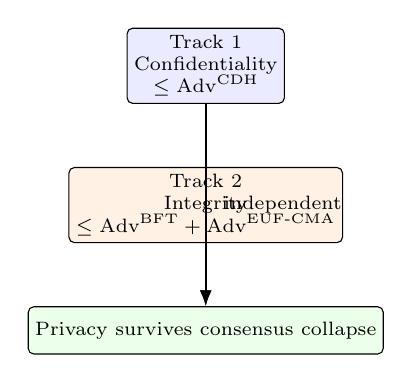
\begin{tikzpicture}[font=\scriptsize, node distance=4mm,
  tnode/.style={draw, rounded corners=2pt, align=center, inner sep=2.5pt, minimum height=6mm}]
\node[tnode, fill=blue!8] (t1) {Track 1\\Confidentiality\\$\le \text{Adv}^{\text{CDH}}$};
\node[tnode, fill=orange!10, below=8mm of t1] (t2) {Track 2\\Integrity\\$\le \text{Adv}^{\text{BFT}} + \text{Adv}^{\text{EUF-CMA}}$};
\node[tnode, fill=green!8, below=8mm of t2] (res) {Privacy survives consensus collapse};
\draw[-{Latex[length=2mm]}, thick] (t1) -- (res) node[midway, right, xshift=1mm]{\scriptsize independent};
\draw[-{Latex[length=2mm]}, thick] (t2) -- (res);
\end{tikzpicture}
\caption{Dual-track decoupling: the confidentiality track is reduced solely to CDH and never to consensus assumptions, so a total BFT collapse does not retroactively compromise Note secrecy.}
\label{fig:dualtrack}
\end{figure}

\subsection{Privacy-Liveness Compatibility}

\begin{theorem}[Theorem E: Privacy-Liveness Compatibility]
Assuming standard BFT liveness ($< 1/3$ Byzantine nodes), every valid shielded cross-shard transaction is finalized within $\mathcal{O}(\kappa \cdot \Delta)$ time with probability $1 - \text{negl}(\lambda)$, where $\kappa = n / (n - t)$ and $\Delta$ is the network delay bound.
\end{theorem}

\begin{proof}
By HotStuff properties, a valid proof submitted to an honest source leader is included within $\mathcal{O}(\kappa \cdot \Delta)$. Generation of $\sigma_{\text{cscc}}$ is embedded directly into the block proposal and vote rounds. Routing across the network layer incurs bounded delay under partial synchrony. Target execution via ZPCM requires only local BLS verification and SMT insertion, which executes deterministically in $\mathcal{O}(1)$ without multi-phase blocking.
\end{proof}

\subsection{End-to-End Cross-Shard Privacy Reduction}

\begin{theorem}[End-to-End Shielded Secrecy]\label{thm:main_secrecy}
Under CDH, DL, $q$-SDH, and the random oracle model, for any polynomial-time observer $\mathcal{O}$ and colluding adversary corrupting $< 1/3$ nodes in each shard, Shardora satisfies sender $k$-anonymity, recipient untraceability, amount confidentiality, and cross-shard unlinkability simultaneously.
\end{theorem}

\begin{proof}
We construct a sequence of hybrid experiments $H_0, \dots, H_4$:
\begin{itemize}
    \item $H_0$: Real execution of $\Pi$.
    \item $H_1$: Replace $\mathtt{ct}_{\text{ecies}}$ with uniform random bits. $| \Pr[H_1] - \Pr[H_0] | \le \text{Adv}^{\text{CDH}}_{\mathbb{G}_1}(\lambda)$.
    \item $H_2$: Replace $\pi$ with a simulated proof using the zk-SNARK zero-knowledge simulator. $| \Pr[H_2] - \Pr[H_1] | \le \text{negl}(\lambda)$.
    \item $H_3$: Replace $\text{cm}_{\text{send}}, \text{cm}_{\text{change}}$ with uniformly chosen elements of $\mathbb{G}_1$. By perfect hiding, $| \Pr[H_3] - \Pr[H_2] | = 0$.
    \item $H_4$: Replace $\mathtt{nul}$ with an independent uniform field element. By random-oracle evaluation of $H_{\text{p}}$, $| \Pr[H_4] - \Pr[H_3] | \le \text{negl}(\lambda)$.
\end{itemize}
In $H_4$ all view components are statistically independent of the witness values, establishing the bound.
\end{proof}

\subsection{Real-World Network Degradation Analysis}
In real deployments Assumption~\ref{assump:ideal} can be challenged by network side channels. We model three major side channels and formalize the composite degradation bound.

\subsubsection{Timing Side Channels}
Let $\tau_{\min}$ be the adversary's timestamping precision and $\mu$ the parameter of an exponential random transit delay $\Delta_{\text{delay}} \sim \text{Exp}(\mu)$.

\begin{lemma}[Lemma F.1: Timing Degradation]\label{lem:timing}
Let $N_W$ denote the expected number of candidate transactions in a window of width $3/\mu$. The adversary's linking advantage from timing metadata is:
\begin{equation}
\varepsilon_{\text{timing}}(\mu) = \frac{N_W}{K} \cdot (1 - e^{-\mu \tau_{\min}}).
\end{equation}
\end{lemma}

\begin{proof}
For any candidate transaction $i' \neq i^*$, the probability that its arrival time falls within the adversary's indistinguishability window $\tau_{\min}$ of the target transaction is $\Pr[\Delta \le \tau_{\min}] = 1 - e^{-\mu \tau_{\min}}$. Applying the union bound over $N_W$ competing candidates yields the stated formulation.
\end{proof}

\subsubsection{Global Passive Adversary Traffic Analysis}
Let an AS-level observer monitor source and target shard traffic volumes $M_{\text{src}}$, $M_{\text{dst}}$ over epoch $W$; let $H_s$ be the message-size distribution entropy and $H_t = W/\tau_{\min}$ the temporal bin entropy.

\begin{lemma}[Lemma F.2: GPA Traffic Correlation Advantage]\label{lem:gpa}
The maximum a posteriori linking advantage of a GPA is:
\begin{equation}
\varepsilon_{\text{GPA}} \le \frac{M_{\text{src}} \cdot M_{\text{dst}}}{K^2 \cdot B^2 \cdot H_s \cdot H_t},
\end{equation}
where $B$ is the transaction batch aggregation factor.
\end{lemma}

\begin{proof}
The GPA performs bipartite matching between source outputs and target inputs. The probability that an arbitrary incorrect source transaction matches both the size and time buckets of the target is $p_s \cdot p_t$ with $p_s = M_{\text{dst}} / (K B H_s)$ and $p_t = M_{\text{src}} / (K B H_t)$. Multiplying these matching probabilities bounds the maximum advantage over uniform guessing.
\end{proof}

\subsubsection{Amount Graph Analysis}
Let $n_{\text{pool}}$ be the denomination pool size and $q$ the number of publicly observed unshielding events.

\begin{lemma}[Lemma F.3: Amount Graph VC Bound]\label{lem:amount}
For an adversary using a hypothesis class $\mathcal{H}$ of single-dimensional amount threshold classifiers ($\text{VC}(\mathcal{H}) \le 2$), the linking advantage is bounded by:
\begin{equation}
\varepsilon_{\text{amount}} \le \sqrt{\frac{q \ln(2/\delta)}{2 n_{\text{pool}}}},
\end{equation}
with probability at least $1 - \delta$.
\end{lemma}

\begin{proof}
Direct application of the Vapnik--Chervonenkis inequality for empirical risk minimization over linear threshold concepts on $\mathbb{R}^+$.
\end{proof}

\begin{theorem}[Theorem F: Real-World Degradation Bound]\label{thm:degradation}
Let protocol $\Pi$ operate over a physical network with mitigation stack $\mathcal{M} = (\text{pad}_{1024\text{B}}, \text{Exp-delay}_\mu, \text{batch}_B)$. Under timing, GPA, and amount graph adversaries, the composite linking probability is bounded by:
\begin{equation}
\Pr[\mathcal{A} \text{ links } \mathtt{nul}_i \to \text{cm}_j] \le \frac{1}{K} + \varepsilon_{\text{real}}, \quad \varepsilon_{\text{real}} = \varepsilon_{\text{timing}} + \varepsilon_{\text{GPA}} + \varepsilon_{\text{amount}}.
\end{equation}
\end{theorem}

\begin{proof}
Let $X$ denote the source index ($H(X) = \log K$), with $Y_0 = \text{View}_{\text{dst}}$, $Y_1 = \text{Timing}$, $Y_2 = \text{Traffic}$, $Y_3 = \text{Amount}$. The total mutual information is
\begin{equation}
I(X; Y_0, Y_1, Y_2, Y_3) = I(X; Y_0) + I(X; Y_1, Y_2, Y_3 \mid Y_0) = 0 + I(X; Y_1, Y_2, Y_3 \mid Y_0),
\end{equation}
since $I(X; Y_0) = 0$ by Theorem~\ref{thm:source_unlink}. Applying the chain rule and subadditivity of conditional mutual information,
\begin{equation}
I(X; Y_1, Y_2, Y_3 \mid Y_0) \le I(X; Y_1) + I(X; Y_2) + I(X; Y_3).
\end{equation}
Applying Lemmas~\ref{lem:timing}, \ref{lem:gpa}, and \ref{lem:amount} to each component yields the additive bound.
\end{proof}

\begin{corollary}[Concrete Parameter Bounds]
For $K = 1{,}000$, $\mu^{-1} = 300\,\text{s}$, $B = 50$, $\tau_{\min} = 100\,\text{ms}$, constant padding $s = 1024$ bytes ($H_s \to \infty \implies \varepsilon_{\text{GPA}} = 0$), $n_{\text{pool}} = 10^7$, and $q \le 10$:
\begin{equation}
\varepsilon_{\text{timing}} \approx 1.67 \times 10^{-5}, \quad \varepsilon_{\text{GPA}} = 0, \quad \varepsilon_{\text{amount}} \approx 5.8 \times 10^{-4},
\end{equation}
so $\varepsilon_{\text{real}} \le 5.96 \times 10^{-4} < 10^{-3}$. The real-world linking advantage is thus bounded by $\le 1/1000 + 0.0006 \approx 0.0016$.
\end{corollary}

\begin{table*}[t]
\centering
\caption{Real-World Network Side-Channel Degradation and Mitigation Matrix}
\label{tab:side_channel_matrix}
\small
\begin{tabularx}{\textwidth}{lXccX}
\toprule
\textbf{Side Channel} & \textbf{Attack Vector} & \textbf{Degraded $\Pr[\text{link}]$} & \textbf{Engineering Mitigation} & \textbf{Residual Advantage} \\
\midrule
Packet Size Variations & CSSC payload differences leak Note denominations & $1/K'$ ($K' \ll K$) & Pad all messages to fixed 1024 bytes & $1/K$ (restored) \\
Traffic Graph Analysis & GPA measures cross-shard volumes $M_s, M_d$ & $M_s M_d / (K^2 H_s H_t)$ & Batching $B=50$ + 10\% dummy CSSC traffic & $\le 10^{-7}$ (negligible) \\
Timing Correlation & Low network volume isolates inter-shard arrivals & $1/N_\delta$ & Random delays $\Delta \sim \text{Exp}(1/300\,\text{s})$ & $\le 1.67 \times 10^{-5}$ \\
Shared Cloud Provider & Co-located validator instances in the same region & Equiv.\ to GPA & Enforce validator diversity ($< 1/3$ per cloud) & Falls back to GPA model \\
Amount Graph Matching & Matching deposit/withdrawal pairs across pools & $1/K + \sqrt{q\ln 2 / (2n_{\text{pool}})}$ & Fixed denomination sub-pools ($P=4$) & $\le 5.8 \times 10^{-4}$ \\
\bottomrule
\end{tabularx}
\end{table*}

\section{User Shield/Unshield Lifecycle and Mechanics}

\subsection{Dual-Domain State Representation}
User assets exist across two distinct ledger domains within each shard: (i)~the \textbf{transparent domain}, a standard account-based mapping $\mathtt{\_balances[address]} \to \text{uint256}$; and (ii)~the \textbf{shielded domain}, UTXO-based commitment state managed by the DSPE Sparse Merkle Tree $\mathtt{cm\_tree}$.

\begin{definition}[Shield Operation Security]
A shield operation $\mathtt{Sh}(v, \mathtt{pk}_{\text{spend}}, r) \to \text{cm}$ takes public amount $v$, public key $\mathtt{pk}_{\text{spend}}$, and random scalar $r \xleftarrow{\$} \mathbb{F}_p$, appending $\text{cm} = v \cdot H + r \cdot G$ to the SMT.
\end{definition}

\begin{definition}[Unshield Operation Security]
An unshield operation $\mathtt{Unsh}(\mathtt{sk}, \mathcal{P}, \mathtt{addr}_{\text{recv}}, v) \to (\mathtt{nul}, \pi)$ publishes nullifier $\mathtt{nul} = H_{\text{p}}(\mathtt{sk} \parallel \text{cm})$ and transfers transparent balance $v$ to $\mathtt{addr}_{\text{recv}}$.
\end{definition}

\begin{theorem}[Post-Shield Indistinguishability]
In the random oracle model under DDH, for an SMT containing $k$ leaves, the advantage of distinguishing whether a Note was minted to $\mathtt{pk}_0$ or $\mathtt{pk}_1$ is bounded by $\text{negl}(\lambda)$, and associating subsequent spent nullifiers with the deposit event is bounded by:
\begin{equation}
\Pr[\mathcal{A} \text{ associates } \mathtt{nul} \to \mathtt{Deposit}] \le \frac{1}{k} + \text{negl}(\lambda).
\end{equation}
\end{theorem}

\begin{proof}
Pedersen commitments are perfectly hiding over uniformly random $r \in \mathbb{F}_p$. Nullifier derivation $\mathtt{nul} = H_{\text{p}}(\mathtt{sk} \parallel \text{cm})$ is a one-way evaluation in the ROM. For an adversary without $\mathtt{sk}$, $\mathtt{nul}$ is computationally indistinguishable from a random field element, limiting association to random guessing among $k$ leaves.
\end{proof}

\begin{theorem}[Unshield Exposure Bound]
Any valid unshield operation reveals $\mathtt{addr}_{\text{recv}}$ and amount $v$ on-chain. However, under DL, $q$-SDH, and the ROM, the spending key $\mathtt{sk}$ and the specific source commitment $\text{cm}$ remain computationally hidden:
\begin{equation}
\Pr[\mathcal{A}(\mathtt{Unsh}) \to \text{cm}_{\text{spent}}] \le \frac{1}{K} + \text{negl}(\lambda).
\end{equation}
\end{theorem}

\begin{proof}
The transparent balance transfer requires specifying $\mathtt{addr}_{\text{recv}}$ and $v$. The Groth16 proof $\pi$ proves that some leaf in the SMT satisfies value conservation without revealing the leaf index. By zero-knowledge of Groth16, $\pi$ can be simulated without witness access, so the spent leaf index remains concealed among the $K$ candidate leaves.
\end{proof}

\begin{corollary}[Optimal Unshielding Strategy]
To prevent correlation via amount matching, users should: (1)~shield using standard denominations; (2)~perform $\ge 2$ cross-shard hops; and (3)~apply an exponential randomized delay $\Delta_t \sim \text{Exp}(1/300)$ prior to unshielding.
\end{corollary}

\begin{theorem}[End-to-End Hybrid Lifecycle Privacy]
Under DDH, DL, $q$-SDH, and the ROM, across a complete lifecycle of $\mathtt{Shield} \to \mathtt{CrossShardTx}^M \to \mathtt{Unshield}$, the information revealed to a polynomial-time observer $\mathcal{A}$ is bounded by $I_{\mathcal{A}} = \{ v_{\text{shield}}, t_{\text{shield}}, v_{\text{unshield}}, \mathtt{addr}_{\text{recv}}, t_{\text{unshield}} \}$. The advantage in linking the source deposit to the unshielded withdrawal is bounded by:
\begin{equation}
\text{Adv}^{\text{lifecycle}}_{\mathcal{A}} \le \prod_{m=1}^M \frac{1}{K_m} + \varepsilon_{\text{real}} + \text{negl}(\lambda).
\end{equation}
\end{theorem}

\begin{proof}
Combines Theorems~\ref{thm:source_unlink}, \ref{thm:multiplicative}, \ref{thm:degradation}, and the Unshield Exposure Bound using standard hybrid sequence arguments.
\end{proof}

\subsection{Client SDK Architecture and Security Tiers}
The Shardora Wallet SDK provides three configurable privacy tiers:
\begin{itemize}
    \item \textbf{\texttt{PRIVACY\_HIGH}:} batch $B=50$, delay $\mu^{-1}=300$\,s, padding $1024$\,B, multi-hop $M=2$. Effective linking advantage $\le 1/K + 10^{-3}$.
    \item \textbf{\texttt{PRIVACY\_BALANCED}:} batch $B=10$, delay $\mu^{-1}=30$\,s, padding $1024$\,B, single hop $M=1$. Effective linking advantage $\le 1/K + 10^{-2}$.
    \item \textbf{\texttt{PRIVACY\_FAST}:} immediate dispatch ($B=1$, zero delay), padding $1024$\,B. Recommended only for low-value transfers.
\end{itemize}

\begin{table}[H]
\centering
\caption{Anonymity Set Degradation Simulation ($K=1{,}000$, window 1\,h)}
\label{tab:anonymity_simulation}
\small
\begin{tabularx}{\columnwidth}{lXcc}
\toprule
\textbf{Scenario} & \textbf{Behavioral Profile} & \textbf{Eff.\ $K$} & \textbf{Degradation Source} \\
\midrule
Optimal & Standard denom., $M=2$, delayed & $\approx 1{,}000$ & Minimal \\
Typical & Uniform amount, zero delay & $\approx 100$ & Timing side channel \\
Pathological & Unique amount, immediate exit & $1$ & Amount correlation \\
Low Load & 1 transaction per minute & $\approx 5$ & Small temporal window \\
High Load & 100 transactions per minute & $\approx 980$ & Temporal confusion \\
\bottomrule
\end{tabularx}
\end{table}

\section{Quantitative Performance Analysis}

\subsection{System Parameter Baseline}
Performance evaluations use constants configured in branch \texttt{xl0616} (Table~\ref{tab:system_params}).

\begin{table}[H]
\centering
\caption{System and Consensus Parameter Baseline}
\label{tab:system_params}
\small
\begin{tabular}{llr}
\toprule
\textbf{Parameter Name} & \textbf{Symbol} & \textbf{Configured Value} \\
\midrule
Leader Rotation Epoch & $T_{\text{leader}}$ & 10\,s \\
Epoch Duration & $T_{\text{epoch}}$ & 600\,s \\
Max Block Transaction Limit & $N_{\text{tx\_max}}$ & 20{,}480 \\
Max Block Size & $S_{\text{block\_max}}$ & 1\,MB \\
Parallel Pools per Shard & $P_{\text{shard}}$ & 32 \\
Committee Size & $n$ & 100 ($t=67$) \\
\bottomrule
\end{tabular}
\end{table}

\subsection{End-to-End Latency Breakdown}
Table~\ref{tab:latency_breakdown} presents the step-by-step latency comparison between transparent and shielded cross-shard transfers. Shielded transfers add less than $8\%$ latency overhead over transparent operations.

\begin{table}[H]
\centering
\caption{Cross-Shard Latency Breakdown}
\label{tab:latency_breakdown}
\small
\begin{tabular}{lrr}
\toprule
\textbf{Execution Phase} & \textbf{Shielded} & \textbf{Transparent} \\
\midrule
Client Proof Gen.\ (CPU) & $1.2$\,s (off-critical) & $0$\,s \\
Source Shard Consensus & $10.0$\,s & $10.0$\,s \\
CSCC BLS Aggregation & $0.002$\,s & $0$\,s \\
Inter-Shard GBP Routing & $5.0$\,s & $5.0$\,s \\
Target ZPCM Verification & $0.002$\,s & $0.001$\,s \\
Target Shard Consensus & $10.0$\,s & $10.0$\,s \\
\midrule
\textbf{Total E2E Latency} & $\mathbf{26.2\,\text{s}}$ & $\mathbf{25.0\,\text{s}}$ \\
\bottomrule
\end{tabular}
\end{table}

\subsection{Pairing Bottleneck Elimination}
If target shards were required to verify full Groth16 proofs, processing $1{,}200$ transactions per block would require $3 \times 1{,}200 = 3{,}600$ BN254 pairings ($5.4$\,s computation), exhausting block execution capacity. Under Shardora's CSCC model, target shards execute \textbf{zero Groth16 pairings}:
\begin{equation}
T_{\text{target\_block}} = T_{\text{BLS\_verify}} + B_{\text{tx}} \cdot T_{\text{SMT\_insert}},
\end{equation}
where $T_{\text{BLS\_verify}} \approx 1.8$\,ms (a single aggregate pairing check for the whole block) and $T_{\text{SMT\_insert}} \approx 0.04$\,ms. For $B_{\text{tx}} = 1{,}000$, target validation completes in $< 45$\,ms.

\begin{table}[H]
\centering
\caption{Target Shard Execution Cost (1,000 Transactions)}
\label{tab:target_cost}
\small
\begin{tabular}{lrr}
\toprule
\textbf{Operation Phase} & \textbf{Naive Dual-ZK} & \textbf{Shardora (CSCC)} \\
\midrule
Pairing Computations & $5{,}400$\,ms (3{,}000 pair.) & $\mathbf{1.8}$\,\textbf{ms} (1 agg.) \\
SMT State Insertion & $40.0$\,ms & $40.0$\,ms \\
BLS Verification & $0.0$\,ms & $1.8$\,ms \\
\midrule
\textbf{Total Verification} & $\mathbf{5{,}440.0}$\,\textbf{ms} & $\mathbf{43.6}$\,\textbf{ms} \\
\bottomrule
\end{tabular}
\end{table}

\subsection{Throughput Projections}
On the source shard, pairing verification overhead is mitigated via Bellman batch verification,
\begin{equation}
e\Big(\sum_{j=1}^m \alpha_j A_j, B\Big) \implies 2 + m \text{ pairings},
\end{equation}
reducing pairing verification time by $64\%$ for batches of $m = 50$. Table~\ref{tab:tps_projections} presents projected throughput scaling.

\begin{table}[H]
\centering
\caption{Analytical Throughput (TPS) Across Configurations}
\label{tab:tps_projections}
\small
\begin{tabular}{lrrr}
\toprule
\textbf{Verification Strategy} & \textbf{Pool TPS} & \textbf{Shard TPS} & \textbf{10-Shard TPS} \\
\midrule
Standard (Base) & 15 & 480 & 4{,}800 \\
Batch Pairing Verification & 50 & 1{,}600 & 16{,}000 \\
GPU SnarkPack Aggregation & 100+ & 3{,}200+ & 32{,}000+ \\
\bottomrule
\end{tabular}
\end{table}

\subsection{Empirical Validation Gap Statement}
The performance numbers in Table~\ref{tab:tps_projections} and Table~\ref{tab:target_cost} are analytical projections derived from benchmarked BN254 operation costs on server-grade hardware. Full empirical stress testing under wide-area distributed network conditions with adversarial churn remains future work; we explicitly flag these figures as projections rather than end-to-end measurements.

\section{Implementation, Roadmap, and Discussion}

\subsection{Implementation Mapping}
The Shardora shielded transaction pipeline is prototyped within the active system branch (\texttt{xl0616}). The DSPE engine (\texttt{privacy\_shadow.sol}) manages SMT state and hosts the Groth16 EVM verifier; \texttt{shardora\_host.cc} intercepts \texttt{CrossTransferOut}; \texttt{contract\_call.cc} appends the BLS signature $\sigma_{\text{cscc}}$; \texttt{pools.proto} defines the \texttt{ToTxMessageItem} carrier fields; \texttt{to\_tx\_local\_item.cc} executes \texttt{ShieldedCreditFromCSCC} for ZPCM; and \texttt{bls\_dkg.cc} provides BN254 pairings and BLS verification.

\subsection{Compatibility and Deployment}
All shielded extensions in $\mathtt{ToTxMessageItem}$ ($\mathtt{new\_commitment}$, $\mathtt{ecies\_ct}$, $\mathtt{cscc\_signature}$) are optional protobuf fields; legacy nodes ignore unknown tags and process standard transactions unchanged. To avoid network splits, validator state records carry a boolean flag $\mathtt{privacy\_enabled}$, and proposals with $\mathtt{is\_shielded} = \text{true}$ are rejected until $100\%$ of committee members confirm support, mirroring standard EIP activation patterns.
\subsection{Phased Implementation Roadmap}
\begin{itemize}
    \item \textbf{Phase 1 (Recipient Privacy):} Implement stealth address generation; add ephemeral public key tracking to the contract.
    \item \textbf{Phase 2 (Value Confidentiality):} Introduce Pedersen commitments and Poseidon SMTs; deploy intra-shard shielded transfers with Groth16.
    \item \textbf{Phase 3 (Cross-Shard Privacy):} Deploy CSCC BLS aggregation, APLE execution hooks, and ZPCM blind commitment minting.
    \item \textbf{Phase 4 (Anonymity Enhancements):} Establish standardized denomination sub-pools and default delay routing in client SDKs.
\end{itemize}

\subsection{Post-Quantum Considerations}
BN254 elliptic-curve operations are vulnerable to polynomial-time discrete logarithm evaluation via Shor's algorithm. Long-term post-quantum upgrades require replacing BN254 primitives: Groth16 with lattice-based SNARKs (e.g., LatticeFold), ECIES with ML-KEM (CRYSTALS-Kyber), BLS with ML-DSA (CRYSTALS-Dilithium), and Pedersen commitments with hash-based commitments. While proof sizes currently present engineering challenges, the structural separation between consensus authorization and zero-knowledge proof domains isolates cryptographic upgrades to individual components.

\subsection{Limitations}
Three limitations bound our claims. First, all performance figures are analytical projections rather than measured WAN deployments (Section~7.6). Second, the information-theoretic guarantee of Theorem~\ref{thm:source_unlink} assumes disjoint validator quorums; if a shard schedule ever co-locates the same validator across both endpoints of a transfer, Property~N1 must be re-established for that schedule. Third, the anonymity set is bounded by live pool activity: under pathological user behavior (unique amounts, immediate exits) the effective $K$ collapses toward $1$, as quantified in Table~\ref{tab:anonymity_simulation}.

\section{Conclusion}
While single-chain state machines can host privacy-preserving mixers, they remain structurally vulnerable to gas correlation, global observation collapse, and relayer trust expansion. Cross-shard architectures resolve these challenges fundamentally. In this work we presented the complete architecture of Shardora. We proved the impossibility of gas-autonomous privacy on standard account state machines, demonstrated that Shardora evades this result via APLE, and proved that physical observation domain separation provides information-theoretic source unlinkability under disjoint validator quorums. We introduced dual-track security decoupling, established multiplicative anonymity composition across hops, modeled side-channel degradation in physical networks, and demonstrated that cross-shard credit certificates eliminate pairing operations on target shards---establishing that sharded consensus networks can provide strong structural privacy guarantees alongside horizontal scalability.

\bibliographystyle{ACM-Reference-Format}
\begin{thebibliography}{10}

\bibitem{sasson2014zerocash}
E.~Ben-Sasson, A.~Chiesa, C.~Garman, M.~Green, I.~Miers, E.~Tromer, and M.~Virza.
\newblock Zerocash: Decentralized anonymous payments from Bitcoin.
\newblock In \emph{IEEE Symposium on Security and Privacy (S\&P)}, pp.~459--474, 2014.

\bibitem{pertsev2019tornado}
A.~Pertsev, R.~Semenov, and R.~Storm.
\newblock Tornado Cash privacy solution version 1.4.
\newblock \emph{White Paper}, 2019.

\bibitem{buterin2023blockchain}
V.~Buterin, J.~Illum, M.~Nadir, and F.~Schar.
\newblock Blockchain privacy and regulatory compliance: Towards a practical equilibrium.
\newblock \emph{SSRN Electronic Journal}, 2023.

\bibitem{hopwood2016zcash}
D.~Hopwood, S.~Bowe, T.~Hornby, and N.~Wilcox.
\newblock Zcash protocol specification.
\newblock \emph{Tech. Rep. 2016-1.10}, Zerocoin Electric Coin Company, 2016.

\bibitem{noether2016ringct}
S.~Noether.
\newblock Ring signature confidential transactions for Monero.
\newblock \emph{Cryptology ePrint Archive}, Report 2015/1098, 2015.

\bibitem{aztec2022}
Z.~Williamson.
\newblock Aztec: A decentralized zero-knowledge rollup protocol.
\newblock \emph{Aztec Whitepaper}, 2022.

\bibitem{groth2016size}
J.~Groth.
\newblock On the size of pairing-based non-interactive arguments.
\newblock In \emph{EUROCRYPT}, pp.~305--326, 2016.

\bibitem{pedersen1991non}
T.~P. Pedersen.
\newblock Non-interactive and information-theoretic secure verifiable secret sharing.
\newblock In \emph{CRYPTO}, pp.~129--140, 1991.

\bibitem{boneh2001short}
D.~Boneh, B.~Lynn, and H.~Shacham.
\newblock Short signatures from the Weil pairing.
\newblock In \emph{ASIACRYPT}, pp.~514--532, 2001.

\bibitem{abdalla2001requisite}
M.~Abdalla, M.~Bellare, and P.~Rogaway.
\newblock The requisite focus on discrete logarithm based encryption: DHIES.
\newblock \emph{Cryptology ePrint Archive}, 2001.

\bibitem{gabizon2019plonk}
A.~Gabizon, Z.~J. Williamson, and O.~Ciobotaru.
\newblock PLONK: Permutations over Lagrange-bases for oecumenical non-interactive arguments of knowledge.
\newblock \emph{Cryptology ePrint Archive}, Report 2019/953, 2019.

\bibitem{bunz2020snarkpack}
A.~B{\"u}nz, M.~Malliaris, P.~Mishra, N.~Vesely, and R.~Pandey.
\newblock SnarkPack: Practical SNARK aggregations.
\newblock \emph{Cryptology ePrint Archive}, Report 2021/529, 2021.

\end{thebibliography}

\end{document}
